%%%%%%%%%%%%%%%%%%%%%%%%%%%%%%%%%%%%%%%%%
% Beamer Presentation
% LaTeX Template
% Version 1.0 (10/11/12)
%
% This template has been downloaded from:
% http://www.LaTeXTemplates.com
%
% License:
% CC BY-NC-SA 3.0 (http://creativecommons.org/licenses/by-nc-sa/3.0/)
%
%%%%%%%%%%%%%%%%%%%%%%%%%%%%%%%%%%%%%%%%%

%----------------------------------------------------------------------------------------
%   PACKAGES AND THEMES
%----------------------------------------------------------------------------------------
\documentclass[aspectratio=169]{beamer}
\usepackage{multicol}
\usepackage{tikz, pgfplots}
\usepackage{enumitem}
\setitemize{label=\usebeamerfont*{itemize item}%
	\usebeamercolor[fg]{itemize item}
	\usebeamertemplate{itemize item}}
%\usepackage{enumerate}

\pgfplotsset{compat=1.5.1}
\usepgfplotslibrary{fillbetween}
\usepackage{tcolorbox}
\resetcounteronoverlays{saveenumi}
\newcounter{saveenumi}
\newcommand{\seti}{\setcounter{saveenumi}{\value{enumi}}}
\newcommand{\conti}{\setcounter{enumi}{\value{saveenumi}}}

\setbeamercovered{transparent}
%\usepackage{enumitem}
\mode<presentation> {

% The Beamer class comes with a number of default slide themes
% which change the colors and layouts of slides. Below this is a list
% of all the themes, uncomment each in turn to see what they look like.

%\usetheme{default}
%\usetheme{AnnArbor}
%\usetheme{Antibes}
%\usetheme{Bergen}
%\usetheme{Berkeley}
%\usetheme{Berlin}
%\usetheme{Boadilla}
%\usetheme{CambridgeUS}
%\usetheme{Copenhagen}
%\usetheme{Darmstadt}
%\usetheme{Dresden}
%\usetheme{Frankfurt}
%\usetheme{Goettingen}
%\usetheme{Hannover}
\usetheme{Ilmenau}
%\usetheme{JuanLesPins}
%\usetheme{Luebeck}
%\usetheme{Madrid}
%\usetheme{Malmoe}
%\usetheme{Marburg}
%\usetheme{Montpellier}
%\usetheme{PaloAlto}
%\usetheme{Pittsburgh}
%\usetheme{Rochester}
%\usetheme{Singapore}
%\usetheme{Szeged}
%\usetheme{Warsaw}

% As well as themes, the Beamer class has a number of color themes
% for any slide theme. Uncomment each of these in turn to see how it
% changes the colors of your current slide theme.

%\usecolortheme{albatross}
%\usecolortheme{beaver}
%\usecolortheme{beetle}
%\usecolortheme{crane}
%\usecolortheme{dolphin}
%\usecolortheme{dove}
%\usecolortheme{fly}
%\usecolortheme{lily}
%\usecolortheme{orchid}
%\usecolortheme{rose}
%\usecolortheme{seagull}
%\usecolortheme{seahorse}
%\usecolortheme{whale}
%\usecolortheme{wolverine}

%\setbeamertemplate{footline} % To remove the footer line in all slides uncomment this line
%\setbeamertemplate{footline}[page number] % To replace the footer line in all slides with a simple slide count uncomment this line
\usefonttheme[onlymath]{serif}

\setbeamertemplate{navigation symbols}{} % To remove the navigation symbols from the bottom of all slides uncomment this line
}
\definecolor{blizzardblue}{rgb}{0.67, 0.9, 0.93}
\newcommand{\Cross}{$\mathbin{\tikz [x=1.4ex,y=1.4ex,line width=.2ex] \draw (0,0) -- (1,1) (0,1) -- (1,0);}$}%

\usepackage{graphicx} % Allows including images
\usepackage{booktabs} % Allows the use of \toprule, \midrule and \bottomrule in tables
\usepackage{mathtools}
\AtBeginSection[]{
	\begin{frame}
		\vfill
		\centering
		\begin{beamercolorbox}[sep=8pt,center,shadow=true,rounded=true]{title}
			\usebeamerfont{title}\insertsectionhead\par%
		\end{beamercolorbox}
		\vfill
	\end{frame}
}

%\usepackage{enumitem}

%----------------------------------------------------------------------------------------
%   TITLE PAGE
%----------------------------------------------------------------------------------------

\title[Signals and Systems - Tutorial \#3]{The Laplace Transform} % The short title appears at the bottom of every slide, the full title is only on the title page

\author{Amirhossein Afsharrad} % Your name

\institute[Sharif University of Technology] % Your institution as it will appear on the bottom of every slide, may be shorthand to save space
{
Signals and Systems\\ 
Tutorial Session 3\\ 
\medskip
 % Your email address
}

\date{\today} % Date, can be changed to a custom date

\begin{document}

\begin{frame}
\titlepage % Print the title page as the first slide
\end{frame}

\begin{frame}
\frametitle{Overview} % Table of contents slide, comment this block out to remove it
\tableofcontents % Throughout your presentation, if you choose to use \section{} and \subsection{} commands, these will automatically be printed on this slide as an overview of your presentation
\end{frame}

%----------------------------------------------------------------------------------------
%   PRESENTATION SLIDES
%----------------------------------------------------------------------------------------

%------------------------------------------------
\section{Introduction} 

\begin{frame}
\frametitle{Introduction}
\begin{block}{Definition}
	The Laplace transform of a continuous-time signal $ x(t) $ is:
		\[X(s) = \int_{-\infty}^{+\infty}x(t)e^{-st}\mathrm{d}t \quad  , \quad s\in\mathbb{C}\ \quad , \quad s = \sigma + j\omega \]
\end{block}
\end{frame}

\begin{frame}
	\frametitle{Example \#1}
		\begin{align*}
		\only<1-> {x_1(t) &= e^{-at}u(t)\\}
		\only<1> {X_1(s) &= \\}
		\only<2-> {X_1(s) &= \int_{-\infty}^{+\infty}x_1(t)e^{-st}\mathrm{d}t\\}
		\only<3-> {&= \int_{-\infty}^{+\infty}e^{-at}e^{-st}u(t)\mathrm{d}t\\}
		\only<4-> {&= \int_{0}^{+\infty}e^{-(a+s)t}\mathrm{d}t\\}
		\only<5> {&= \frac{-1}{a+s}e^{-(s+a)t}\Big|_0^\infty\\}
		\only<6> {&= \frac{-1}{a+s}e^{-(s+a)t}\Big|_0^\infty =\frac{1}{s+a}\\}
		\only<7> {&= \frac{-1}{a+s}e^{-(s+a)t}\Big|_0^\infty =\frac{1}{s+a} \quad, \quad \textcolor{red}{\mathbf{Re}\{s\}>-\mathbf{Re}\{a\}}\\}
		\end{align*}
\end{frame}

\begin{frame}
\frametitle{Example \#2}
\begin{align*}
		\only<1-> {x_2(t) &= -e^{-at}u(-t)\\}
		\only<1> {X_1(s) &= \\}
		\only<2> {X_1(s) &= \int_{-\infty}^{+\infty}x_2(t)e^{-st}\mathrm{d}t\\}
		\only<3-> {&= \int_{-\infty}^{+\infty}x_2(t)e^{-st}\mathrm{d}t= \int_{-\infty}^{+\infty}-e^{-at}e^{-st}u(-t)\mathrm{d}t\\}
		\only<4> {&= \int_{-\infty}^{0}-e^{-(s+a)t}\mathrm{d}t\\}
		\only<5-> {&= \int_{-\infty}^{0}-e^{-(s+a)t}\mathrm{d}t= \int_{0}^{+\infty}-e^{(s+a)t}\mathrm{d}t\\}
		%\only<5> {&= \frac{-1}{a+s}e^{-(s+a)t}\Big|_0^\infty\\}
		\only<6> {&= \frac{-1}{s+a}e^{(s+a)t}\Big|_0^\infty =\frac{1}{s+a}\\}
		\only<7> {&= \frac{-1}{s+a}e^{(s+a)t}\Big|_0^\infty =\frac{1}{s+a} \quad, \quad \textcolor{red}{\mathbf{Re}\{s\}<-\mathbf{Re}\{a\}}\\}
\end{align*}
\end{frame}



\begin{frame}{Summary - Examples \#1 and \#2}	
	\begin{columns}
		\column{.5\linewidth}
		\[x_1(t) = e^{-at}u(t)\]
		\[X_1(s) = \frac{1}{s+a}\]
		\[\mathbf{Re}\{s\}>-\mathbf{Re}\{a\}\]
		\only<1>{\begin{figure}
				\begin{tikzpicture}
				\begin{axis}
				[
				axis y line=middle,
				axis x line=middle,
				xlabel = {$ t $},
				ylabel = {$ x_1(t) $},
				xtick style={draw=none},
				ytick style={draw=none},
				y=1cm/1,
				x=1cm/1,
				xmin=-2.5,
				xmax=2.5,
				ymin=-.2,
				ymax=2,
				yticklabels={,,},
				xticklabels={,,},
				%			xtick={1},
				ticklabel style={xshift=0.7ex}
				]
				%			\draw [name path=A,dashed, blue, thick, fill = blue, fill opacity = .2](axis cs:0,0) circle [radius=1.25];
				\addplot[domain=0:2.3, samples=100, thick, color = blue]
				{exp(-2*x)};
				\addplot[domain=-2.3:0, samples=100, thick, color = blue]
				{0};
				\draw [blue, thick] (axis cs:0,0) -- (axis cs:0,1);

				\end{axis}
				\end{tikzpicture}
			\end{figure}
		}
			
		
		\column{.5\linewidth}
		\[x_2(t) = -e^{-at}u(-t)\]
		\[X_2(s) = \frac{1}{s+a}\]
		\[\mathbf{Re}\{s\}<-\mathbf{Re}\{a\}\]
				\only<1>{\begin{figure}
						\begin{tikzpicture}
						\begin{axis}
						[
						axis y line=middle,
						axis x line=middle,
						xlabel = {$ t $},
						ylabel = {$ x_2(t) $},
						xtick style={draw=none},
						ytick style={draw=none},
						y=1cm/1,
						x=1cm/1,
						xmin=-2.5,
						xmax=2.5,
						ymin=-2,
						ymax=.8,
						yticklabels={,,},
						xticklabels={,,},
						%			xtick={1},
						ticklabel style={xshift=0.7ex}
						]
						%			\draw [name path=A,dashed, blue, thick, fill = blue, fill opacity = .2](axis cs:0,0) circle [radius=1.25];
						\addplot[domain=-2.3:0, samples=100, thick, color = blue]
						{-exp(-x/3)};
						\addplot[domain=0:2.3, samples=100, thick, color = blue]
						{0};
						\draw [blue, thick] (axis cs:0,0) -- (axis cs:0,-1);
						\end{axis}
						\end{tikzpicture}
					\end{figure}
		}
		
	\end{columns}
\only<2->{\vspace{1cm}
		\begin{itemize}
	\item <2->
	Note that $ X_1(s) = X_2(s) $ while $ x_1(t) \neq x_2(t) $.
	\item <3> The Laplace transform is not unique without specifying where $ X(s) $ is defined.
	\end{itemize}}
\end{frame}

\begin{frame}{The Region of Convergence}
	\onslide<1->\begin{block}{Definition}
		The region of the complex plane for which the Laplace transform $ X(s) $ is defined is called the \textbf{Region Of Convergence (ROC)}.
	\end{block}

	\onslide<2->\begin{block}{Remark}
		The Laplace transform of a continuous-time signal is a pair $ \left(X(s) , \mathrm{ROC}\right) $. To answer the question "Find the Laplace transform of the signal $ x(t) $", reporting $ X(s) $ without specifying the ROC is \textbf{an incomplete answer}.
	\end{block}
\end{frame}

\begin{frame}{The Inverse Laplace Transform}
	The following equation for the inverse Laplace transform is \textit{rarely} used.
	\begin{block}{Formula}
		\[x(t) = \frac{1}{2\pi j}\int_{\sigma-j\infty}^{\sigma+j\infty}X(s)e^{st}\mathrm{d}s\]
	\end{block}
	The value of $ \sigma $ can be chosen as any value for which $ X(s) $ converges -- i.e., any value such that the straight line of integration $ \mathbf{Re}(s) = \sigma $
	is in the ROC.
\end{frame}

\section{Properties of the ROC}
\begin{frame}{Properties of the ROC}
	\begin{block}{Property 1}
		The ROC of $ X(s) $ consists of strips parallel to the $ j\omega $-axis in the $ s $-plane.
	\end{block}
\begin{columns}
	
\column{.33\linewidth}
\begin{figure}[h!]
	\centering
	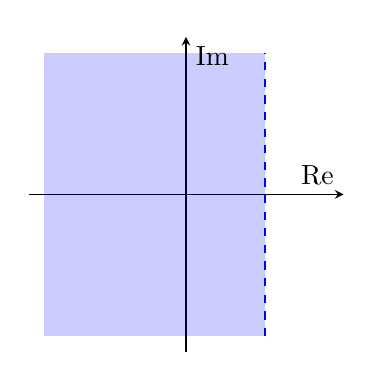
\begin{tikzpicture}
	\begin{axis}
	[
	axis y line=middle,
	axis x line=middle,
	xlabel = {Re},
	ylabel = {Im},
	xtick style={draw=none},
	ytick style={draw=none},
	y=1cm/1,
	x=1cm/1,
	xmin=-2,
	xmax=2,
	ymin=-2,
	ymax=2,
	yticklabels={,,},
	xticklabels={,,},
	%			xtick={1},
	ticklabel style={xshift=0.7ex}
	]
	\draw [name path=A, blue, draw = none, fill = blue, fill opacity = .2](axis cs:-1.8,-1.8) rectangle (axis cs: 1,1.8);
	\draw [blue, thick, dashed] (axis cs: 1,-1.8) -- (axis cs: 1,1.8);
	\end{axis}
	\end{tikzpicture}
\end{figure}
	
	\column{.33\linewidth}
			\begin{figure}[h!]
		\centering
		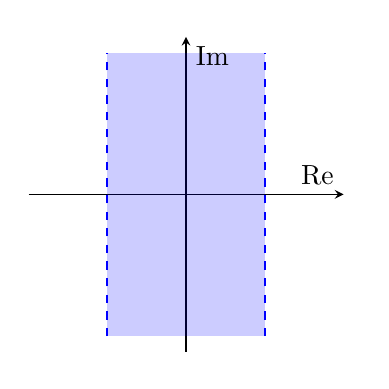
\begin{tikzpicture}
		\begin{axis}
		[
		axis y line=middle,
		axis x line=middle,
		xlabel = {Re},
		ylabel = {Im},
		xtick style={draw=none},
		ytick style={draw=none},
		y=1cm/1,
		x=1cm/1,
		xmin=-2,
		xmax=2,
		ymin=-2,
		ymax=2,
		yticklabels={,,},
		xticklabels={,,},
		%			xtick={1},
		ticklabel style={xshift=0.7ex}
		]
		\draw [name path=A, blue, draw = none, fill = blue, fill opacity = .2](axis cs:-1,-1.8) rectangle (axis cs: 1,1.8);
		\draw [blue, thick, dashed] (axis cs: 1,-1.8) -- (axis cs: 1,1.8);
		\draw [blue, thick, dashed] (axis cs: -1,-1.8) -- (axis cs: -1,1.8);
		\end{axis}
		\end{tikzpicture}
	\end{figure}

	\column{.33\linewidth}
\begin{figure}[h!]
	\centering
	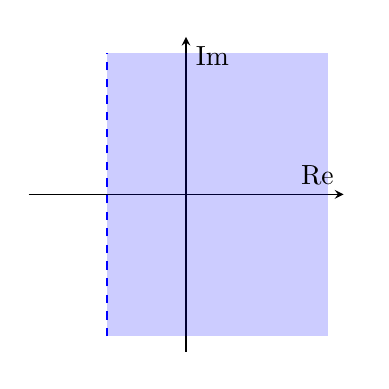
\begin{tikzpicture}
	\begin{axis}
	[
	axis y line=middle,
	axis x line=middle,
	xlabel = {Re},
	ylabel = {Im},
	xtick style={draw=none},
	ytick style={draw=none},
	y=1cm/1,
	x=1cm/1,
	xmin=-2,
	xmax=2,
	ymin=-2,
	ymax=2,
	yticklabels={,,},
	xticklabels={,,},
	%			xtick={1},
	ticklabel style={xshift=0.7ex}
	]
	\draw [name path=A, blue, draw = none, fill = blue, fill opacity = .2](axis cs:-1,-1.8) rectangle (axis cs: 1.8,1.8);
	\draw [blue, thick, dashed] (axis cs: -1,-1.8) -- (axis cs: -1,1.8);
	\end{axis}
	\end{tikzpicture}
\end{figure}
		
	\end{columns}
\end{frame}

\begin{frame}{Properties of the ROC}
	\begin{block}{Property 2}
		For rational Laplace transforms, the ROC does not contain any poles.
	\end{block}
\end{frame}

\begin{frame}{Properties of the ROC}
	\begin{block}{Property 3}
		If $ x(t) $ is of finite duration and is absolutely integrable, then the ROC is
		the entire $ s $-plane.
	\end{block}
\end{frame}

\begin{frame}{Properties of the ROC}
	\begin{columns}
	\column{.66\linewidth}	
		\begin{block}{Property 4}
		If $ x(t) $ is right-sided, and if the line $ \mathbf{Re}\{s\}=\sigma_0 $ is in the ROC, then all
values of $ s $ for which $ \mathbf{Re}\{s\}>\sigma_0 $ will also be in the ROC.
	\end{block}
	
	\begin{definition}
		The signal $ x[n] $ or $ x(t) $ is called \textbf{right-sided} if:
		\[\exists n_0 \: , \: \forall n < n_0 \: : \: x[n] = 0\]
		\[\exists t_0 \: , \:\forall t < t_0 \: : \: x(t) = 0\]
	\end{definition}
		
	\column{.33\linewidth}
		\begin{figure}[h!]
			\centering
			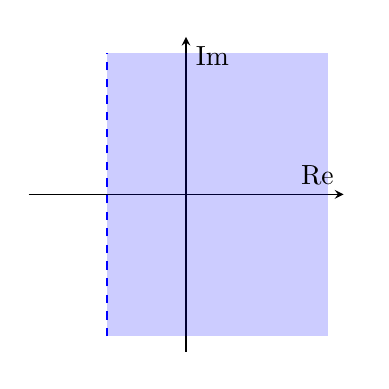
\begin{tikzpicture}
			\begin{axis}
			[
			axis y line=middle,
			axis x line=middle,
			xlabel = {Re},
			ylabel = {Im},
			xtick style={draw=none},
			ytick style={draw=none},
			y=1cm/1,
			x=1cm/1,
			xmin=-2,
			xmax=2,
			ymin=-2,
			ymax=2,
			yticklabels={,,},
			xticklabels={,,},
			%			xtick={1},
			ticklabel style={xshift=0.7ex}
			]
			\draw [name path=A, blue, draw = none, fill = blue, fill opacity = .2](axis cs:-1,-1.8) rectangle (axis cs: 1.8,1.8);
			\draw [blue, thick, dashed] (axis cs: -1,-1.8) -- (axis cs: -1,1.8);
			\end{axis}
			\end{tikzpicture}
		\end{figure}
		
	\end{columns}

\end{frame}


\begin{frame}{Properties of the ROC}
	\begin{columns}
		\column{.66\linewidth}	
	\begin{block}{Property 5}
	If $ x(t) $ is left sided, and if the line $ \mathbf{Re}\{s\}=\sigma_0 $ is in the ROC, then all
values of $ s $ for which $ \mathbf{Re}\{s\}<\sigma_0 $ will also be in the ROC.
	\end{block}
	
	\begin{definition}
		The signal $ x[n] $ or $ x(t) $ is called \textbf{left-sided} if:
		\[\exists n_0 \: , \: \forall n > n_0 \: : \: x[n] = 0\]
		\[\exists t_0 \: , \:\forall t > t_0 \: : \: x(t) = 0\]
	\end{definition}

		
		\column{.33\linewidth}
		\begin{figure}
			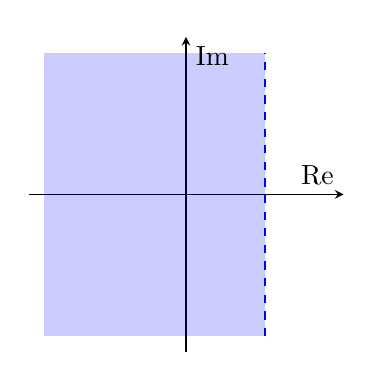
\begin{tikzpicture}
		\begin{axis}
		[
		axis y line=middle,
		axis x line=middle,
		xlabel = {Re},
		ylabel = {Im},
		xtick style={draw=none},
		ytick style={draw=none},
		y=1cm/1,
		x=1cm/1,
		xmin=-2,
		xmax=2,
		ymin=-2,
		ymax=2,
		yticklabels={,,},
		xticklabels={,,},
		%			xtick={1},
		ticklabel style={xshift=0.7ex}
		]
		\draw [name path=A, blue, draw = none, fill = blue, fill opacity = .2](axis cs:-1.8,-1.8) rectangle (axis cs: 1,1.8);
		\draw [blue, thick, dashed] (axis cs: 1,-1.8) -- (axis cs: 1,1.8);
		\end{axis}
		\end{tikzpicture}
		\end{figure}
	\end{columns}
	
\end{frame}

\begin{frame}{Properties of the ROC}
	\begin{columns}
		\column{.66\linewidth}	
		\begin{block}{Property 6}
			If $ x(t) $ is two sided, and if the line $ \mathbf{Re}\{s\}=\sigma_0 $ is in the ROC, then the
ROC will consist of a strip in the $ s $-plane that includes the line $ \mathbf{Re}\{s\}=\sigma_0 $.
		\end{block}
		
		
		\begin{definition}
			The signal $ x[n] $ or $ x(t) $ is called \textbf{two sided} if it is neither left-sided nor right-sided.
		\end{definition}
		
		
		\column{.33\linewidth}
		\begin{figure}[h!]
			\centering
			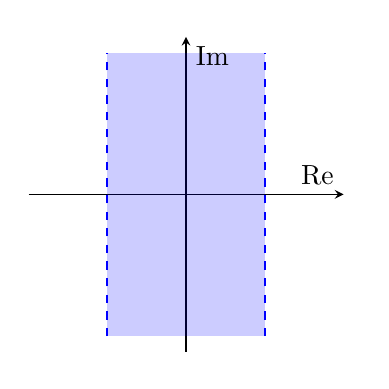
\begin{tikzpicture}
			\begin{axis}
			[
			axis y line=middle,
			axis x line=middle,
			xlabel = {Re},
			ylabel = {Im},
			xtick style={draw=none},
			ytick style={draw=none},
			y=1cm/1,
			x=1cm/1,
			xmin=-2,
			xmax=2,
			ymin=-2,
			ymax=2,
			yticklabels={,,},
			xticklabels={,,},
			%			xtick={1},
			ticklabel style={xshift=0.7ex}
			]
			\draw [name path=A, blue, draw = none, fill = blue, fill opacity = .2](axis cs:-1,-1.8) rectangle (axis cs: 1,1.8);
			\draw [blue, thick, dashed] (axis cs: 1,-1.8) -- (axis cs: 1,1.8);
			\draw [blue, thick, dashed] (axis cs: -1,-1.8) -- (axis cs: -1,1.8);
			\end{axis}
			\end{tikzpicture}
		\end{figure}
		
	\end{columns}
	
\end{frame}

\begin{frame}{Properties of the ROC}
	\begin{block}{Property 7}
		If the Laplace transform $ X(s) $ of $ x(t) $ is rational, then its ROC is bounded
		by poles or extends to infinity. In addition, no poles of $ X(s) $ are contained in the ROC.
	\end{block}
\end{frame}

\begin{frame}{Properties of the ROC}
	\begin{block}{Property 8}
		If the Laplace transform $ X(s) $ of $ x(t) $ is rational, then if $ x(t) $ is right sided,
the ROC is the region in the $ s $-plane to the right of the rightmost pole. If $ x(t) $ is left sided,
the ROC is the region in the $ s $-plane to the left of the leftmost pole.
	\end{block}
\end{frame}

\begin{frame}{Example \#3}

	\[X(s)=\frac{2(s+2)}{s^2+7s+12}\Rightarrow x(t)=?\]
	\begin{columns}
		\column{.4\linewidth}
	\begin{align*}
		\only<2->{ X(z) &= \frac{2(s+2)}{(s+3)(s+4)}\\}
		\only<3->{ &= \frac{4}{s+4}-\frac{2}{s+3}\\}
	\end{align*}
	\column{.05\linewidth}
	\only<5->{\[\Rightarrow\]}
	\column{.55\linewidth}
	\only<4>{
		\textbf{Do you remember the results from examples \#1 and \#2?}
	}
	\only<5->{
		\[x(t) = \begin{cases}
		 4e^{-4t}u(t)-2e^{-3t}u(t)\\
		 4e^{-4t}u(t)+2e^{-3t}u(-t)\\
		-4e^{-4t}u(-t)+2e^{-3t}u(-t) \\
		\textcolor{red}{-4e^{-4t}u(-t)-2e^{-3t}u(t)}
		\end{cases}\]
	}
	\end{columns}
\end{frame}

\begin{frame}{Example \#3}
\only<1>{
	\[X(s)=\frac{2(s+2)}{s^2+7s+12}\Rightarrow x(t)=4e^{-4t}u(t)-2e^{-3t}u(t)\]
		\begin{figure}[h!]
			\centering
			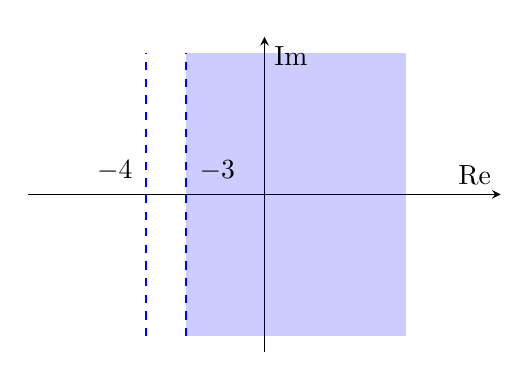
\begin{tikzpicture}
			\begin{axis}
			[
			axis y line=middle,
			axis x line=middle,
			xlabel = {Re},
			ylabel = {Im},
			xtick style={draw=none},
			ytick style={draw=none},
			y=1cm/1,
			x=1cm/1,
			xmin=-3,
			xmax=3,
			ymin=-2,
			ymax=2,
			yticklabels={,,},
			xticklabels={,,},
			%			xtick={1},
			ticklabel style={xshift=0.7ex}
			]
			\draw [name path=A, blue, draw = none, fill = blue, fill opacity = .2](axis cs:-1,-1.8) rectangle (axis cs: 1.8,1.8);
			\draw [blue, thick, dashed] (axis cs: -1,-1.8) -- (axis cs: -1,1.8);
			\draw [blue, thick, dashed] (axis cs: -1.5,-1.8) -- (axis cs: -1.5,1.8);
			\draw (axis cs: -1.9,.3) node {$ -4 $};
			\draw (axis cs: -.6,.3) node {$ -3 $};
			\end{axis}
			\end{tikzpicture}
		\end{figure}
}
\only<2>{
	\[X(s)=\frac{2(s+2)}{s^2+7s+12}\Rightarrow x(t)=4e^{-4t}u(t)+2e^{-3t}u(-t)\]
	\begin{figure}[h!]
		\centering
		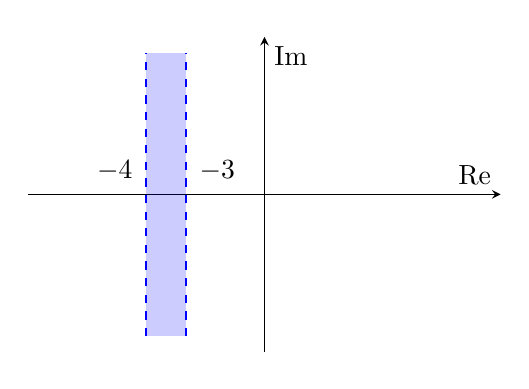
\begin{tikzpicture}
		\begin{axis}
		[
		axis y line=middle,
		axis x line=middle,
		xlabel = {Re},
		ylabel = {Im},
		xtick style={draw=none},
		ytick style={draw=none},
		y=1cm/1,
		x=1cm/1,
		xmin=-3,
		xmax=3,
		ymin=-2,
		ymax=2,
		yticklabels={,,},
		xticklabels={,,},
		%			xtick={1},
		ticklabel style={xshift=0.7ex}
		]
		\draw [name path=A, blue, draw = none, fill = blue, fill opacity = .2](axis cs:-1.5,-1.8) rectangle (axis cs: -1,1.8);
		\draw [blue, thick, dashed] (axis cs: -1,-1.8) -- (axis cs: -1,1.8);
		\draw [blue, thick, dashed] (axis cs: -1.5,-1.8) -- (axis cs: -1.5,1.8);
		\draw (axis cs: -1.9,.3) node {$ -4 $};
		\draw (axis cs: -.6,.3) node {$ -3 $};
		\end{axis}
		\end{tikzpicture}
	\end{figure}
}
\only<3>{
	\[X(s)=\frac{2(s+2)}{s^2+7s+12}\Rightarrow x(t)=-4e^{-4t}u(-t)+2e^{-3t}u(-t)\]
	\begin{figure}[h!]
		\centering
		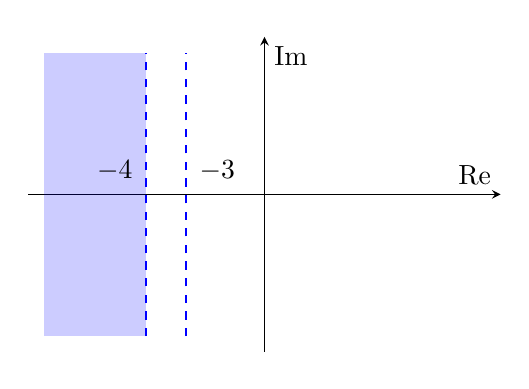
\begin{tikzpicture}
		\begin{axis}
		[
		axis y line=middle,
		axis x line=middle,
		xlabel = {Re},
		ylabel = {Im},
		xtick style={draw=none},
		ytick style={draw=none},
		y=1cm/1,
		x=1cm/1,
		xmin=-3,
		xmax=3,
		ymin=-2,
		ymax=2,
		yticklabels={,,},
		xticklabels={,,},
		%			xtick={1},
		ticklabel style={xshift=0.7ex}
		]
		\draw [name path=A, blue, draw = none, fill = blue, fill opacity = .2](axis cs:-2.8,-1.8) rectangle (axis cs: -1.5,1.8);
		\draw [blue, thick, dashed] (axis cs: -1,-1.8) -- (axis cs: -1,1.8);
		\draw [blue, thick, dashed] (axis cs: -1.5,-1.8) -- (axis cs: -1.5,1.8);
		\draw (axis cs: -1.9,.3) node {$ -4 $};
		\draw (axis cs: -.6,.3) node {$ -3 $};
		\end{axis}
		\end{tikzpicture}
	\end{figure}
}
\only<4>{
	\[X(s)=\frac{2(s+2)}{s^2+7s+12}\Rightarrow x(t)=-4e^{-4t}u(-t)-2e^{-3t}u(t)\]
	\begin{figure}[h!]
		\centering
		\begin{tikzpicture}
		\begin{axis}
		[
		axis y line=middle,
		axis x line=middle,
		xlabel = {Re},
		ylabel = {Im},
		xtick style={draw=none},
		ytick style={draw=none},
		y=1cm/1,
		x=1cm/1,
		xmin=-3,
		xmax=3,
		ymin=-2,
		ymax=2,
		yticklabels={,,},
		xticklabels={,,},
		%			xtick={1},
		ticklabel style={xshift=0.7ex}
		]
		\draw [blue, thick, dashed] (axis cs: -1,-1.8) -- (axis cs: -1,1.8);
		\draw [blue, thick, dashed] (axis cs: -1.5,-1.8) -- (axis cs: -1.5,1.8);
		\draw (axis cs: -1.9,.3) node {$ -4 $};
		\draw (axis cs: -.6,.3) node {$ -3 $};
		\end{axis}
		\end{tikzpicture}
	\end{figure}
}
\end{frame}



\section{Properties of the Laplace Transform}
\begin{frame}{Linearity}
	If\\
	 \[x_1(t) \xleftrightarrow[]{\quad\mathcal{L}\quad} X_1(s) \text{, with } \mathrm{ROC} =R_1\]
	and\\
	\[ x_2(t) \xleftrightarrow[]{\quad\mathcal{L}\quad} X_2(s) \text{, with   } \mathrm{ROC} =R_2 \]
	then
	\begin{block}{Property 1}
		\[ ax_1(t)+bx_2(t) \xleftrightarrow[]{\quad\mathcal{L}\quad} aX_1(s)+bX_2(s)\]  
		\centering
		with ROC containing  $ R_1\cap R_2 $ 
	\end{block}
\end{frame}

\begin{frame}{Time Shifting}
	If\\
	\[x(t) \xleftrightarrow[]{\quad\mathcal{L}\quad} X(s) \text{, with } \mathrm{ROC} =R\]
	then
	\begin{block}{Property 2}
		\[ x(t-t_0) \xleftrightarrow[]{\quad\mathcal{L}\quad} e^{-st_0}X(s) \]
		\centering
		 with $\mathrm{ROC} = R $
	\end{block}
\end{frame}

\begin{frame}{Shifting in the $ s $-Domain}
If\\
\[x(t) \xleftrightarrow[]{\quad\mathcal{L}\quad} X(s) \text{, with } \mathrm{ROC} =R\]
then
\begin{block}{Property 3}
	\[ e^{s_0t}x(t) \xleftrightarrow[]{\quad\mathcal{L}\quad} X(s-s_0) \]
	\centering
	with $\mathrm{ROC} = R + \mathbf{Re}\{s_0\} $
\end{block}
\end{frame}

\begin{frame}{Time Scaling}
If\\
\[x(t) \xleftrightarrow[]{\quad\mathcal{L}\quad} X(s) \text{, with } \mathrm{ROC} =R\]
then
\begin{block}{Property 4}
	\[ x(at) \xleftrightarrow[]{\quad\mathcal{L}\quad} \frac{1}{|a|}X\left(\frac{s}{a}\right) \]
	\centering
	with $\mathrm{ROC} = |a|R $
\end{block}
\end{frame}

\begin{frame}{Conjugation}
If\\
\[x(t) \xleftrightarrow[]{\quad\mathcal{L}\quad} X(s) \text{, with } \mathrm{ROC} =R\]
then
\begin{block}{Property 5}
	\[ x^*(t) \xleftrightarrow[]{\quad\mathcal{L}\quad} X^*(s^*) \]
	\centering
	with $\mathrm{ROC} = R $
\end{block}
\end{frame}

\begin{frame}{Convolution Property}
If\\
\[x_1(t) \xleftrightarrow[]{\quad\mathcal{L}\quad} X_1(s) \text{, with } \mathrm{ROC} =R_1\]
	and\\
\[ x_2(t) \xleftrightarrow[]{\quad\mathcal{L}\quad} X_2(s) \text{, with   } \mathrm{ROC} =R_2 \]
then
\begin{block}{Property 6}
	\[ x_1(t)*x_2(t) \xleftrightarrow[]{\quad\mathcal{L}\quad} X_1(s)X_2(s) \]
	\centering
	with ROC containing  $ R_1\cap R_2 $ 
\end{block}
\end{frame}

\begin{frame}{Differentiation in the Time Domain}
If\\
\[x(t) \xleftrightarrow[]{\quad\mathcal{L}\quad} X(s) \text{, with } \mathrm{ROC} =R\]
then
\begin{block}{Property 7}
	\[ \frac{\mathrm{d}x(t)}{\mathrm{d}t} \xleftrightarrow[]{\quad\mathcal{L}\quad} sX(s) \]
	\centering
	with ROC containing $ R $
\end{block}
\end{frame}

\begin{frame}{Differentiation in the $ s $ - Domain}
If\\
\[x(t) \xleftrightarrow[]{\quad\mathcal{L}\quad} X(s) \text{, with } \mathrm{ROC} =R\]
then
\begin{block}{Property 8}
	\[ -tx(t) \xleftrightarrow[]{\quad\mathcal{L}\quad} \frac{\mathrm{d}X(s)}{\mathrm{d}s} \]
	\centering
	with $\mathrm{ROC} = R $
\end{block}
\end{frame}

\begin{frame}{Integration in the Time Domain}
If\\
\[x(t) \xleftrightarrow[]{\quad\mathcal{L}\quad} X(s) \text{, with } \mathrm{ROC} =R\]
then
\begin{block}{Property 9}
	\[ \int_{-\infty}^{t}x(\tau)\mathrm{d}\tau \xleftrightarrow[]{\quad\mathcal{L}\quad} \frac{1}{s}X(s) \]
	\centering
	with ROC containing $ R\cap\{\mathbf{Re}\{s\}>0\} $
\end{block}
\end{frame}

\begin{frame}{The Initial Value Theorem}
If $ x(t) = 0 $ for $ t<0 $ and $ x(t) $ contains no impulses or higher order singularities at the origin, then 
\begin{block}{Property 10}
	\[\lim\limits_{t\to 0^+}x(t) = \lim\limits_{s\to\infty}sX(s)\]
\end{block}
\end{frame}

\begin{frame}{The Final Value Theorem}
If $ x(t) = 0 $ for $ t<0 $ and $ x(t) $ has a finite limit as $ t\to \infty $, then 
\begin{block}{Property 10}
	\[\lim\limits_{t\to \infty}x(t) = \lim\limits_{s\to0}sX(s)\]
\end{block}

\end{frame}

\begin{frame}{Example \#4}
\only<1>{
	Suppose the following facts are given about the signal $ x(t) $ with Laplace transform $ X(s) $:
	\begin{itemize}
		\item $ x(t) $ is real and even.
		\item $ X(s) $ has four poles and no zeros in the finite $ s $-plane.
		\item $ X(s) $ has a pole at $ s = \left(\frac{1}{2}\right)e^{j\pi/4} $.
		\item $ \int_{-\infty}^{\infty}x(t)\mathrm{d}t = 4 $
	\end{itemize}	
Determine $ X(s) $ and its ROC.
}

\only<2>{
	\[p_1 = \left(\frac{1}{2}\right)e^{j\pi/4} \]
	\[p_2 = \left(\frac{1}{2}\right)e^{-j\pi/4} \]
	\[p_3 = -\left(\frac{1}{2}\right)e^{j\pi/4} \]
	\[p_4 = -\left(\frac{1}{2}\right)e^{-j\pi/4} \]
	\[X(s) = \frac{K}{(s^2-\frac{1}{\sqrt{2}}s+\frac{1}{4})(s^2+\frac{1}{\sqrt{2}}s+\frac{1}{4})}\]
}
\only<3>{
	\[X(s) = \frac{K}{(s^2-\frac{1}{\sqrt{2}}s+\frac{1}{4})(s^2+\frac{1}{\sqrt{2}}s+\frac{1}{4})}\]
	\[\int_{-\infty}^{\infty}x(t)\mathrm{d}t = 4\]
	\[\Rightarrow X(s) = \frac{\frac{1}{4}}{(s^2-\frac{1}{\sqrt{2}}s+\frac{1}{4})(s^2+\frac{1}{\sqrt{2}}s+\frac{1}{4})}\]
	\[\mathrm{ROC}:\quad -\frac{1}{2}<\mathbf{Re}\{s\}<\frac{1}{2}\]
}
\end{frame}


\section{The Laplace Transform and LTI Systems}
\begin{frame}{System Transfer Function}
	The input-output relationship for an LTI system with impulse response $ h(t) $:
	\[y(t) = h(t)*x(t)\]
	Using the convolution property of the Laplace transform:
	\[Y(s) = H(s)X(s)\]
	\[H(s) = \frac{Y(s)}{X(s)}\]
	\begin{block}{Definition}
		$ H(s) $ is called the \textbf{transfer function} (or \textbf{system function}) of the system.
	\end{block}
	Note that $ H(s) $ is the Laplace transform of the impulse response of the system.
\end{frame}

\begin{frame}{Causality of LTI Systems}
	\begin{block}{Theorem}
		The ROC associated with the system function for a
causal LTI system is a right-half plane.
	\end{block}
Note that the converse of this statement is not necessarily true. That is, an ROC to the right of the rightmost pole does not guarantee that a system is causal; rather, it guarantees only that the impulse
response is right sided.\\
%\begin{itemize}
%	\item Example:
%\end{itemize}

\[h(t) = e^{-(t+1)}u(t+1)\Rightarrow H(s) = \frac{e^s}{s+1} \quad,\quad \mathbf{Re}\{s\}>-1\]


\end{frame}

\begin{frame}{Causality of LTI Systems}
\begin{block}{Theorem}
	For a system with a rational system function, causality
of the system is equivalent to the ROC being the
right-half plane to the right of the rightmost pole.
	
\end{block}
\end{frame}


\begin{frame}{Stability of LTI Systems}
\begin{block}{Theorem}
	An LTI system is stable if and only if the ROC
of its system function $ H(s) $ includes the entire
$ jw $-axis [i.e., $ \mathbf{Re}\{s\} = 0 $].
\end{block}
\end{frame}



	\begin{frame}{Example \#5}
		\only<1>{
		Find the impulse response of the system described by the differential equation
		\[\frac{\mathrm{d}^2y(t)}{\mathrm{d}t^2}-\frac{\mathrm{d}y(t)}{dt}-2y(t)=x(t)\]
		if the system is:
		\begin{enumerate}[label=(\alph*)]
			\item stable.
			\item causal.
			\item non-causal and unstable.
		\end{enumerate}}
		\only<2-4>{
		\[\frac{\mathrm{d}^2y(t)}{\mathrm{d}t^2}-\frac{\mathrm{d}y(t)}{dt}-2y(t)=x(t)\]
		\[s^2Y(s)-sY(s)-2Y(s) = X(s)\]
	}
\only<3-4>{
	\begin{align*}
		\only<3-4>{
			H(s) = \frac{Y(s)}{X(s)} &= \frac{1} {s^2-s-2}\\
		}
		\only<4-4>{ &= \frac{1/3}{s-2} - \frac{1/3}{s+1}}
	\end{align*}
}
%\end{frame}
%\begin{frame}
	\only<5>{
		\begin{columns}
			\column{.5\textwidth}
			For a stable system:
			\[H(s) = \frac{1/3}{s-2} - \frac{1/3}{s+1}\]
			\[h(t) = -\frac{1}{3}e^{2t}u(-t) - \frac{1}{3}e^{-t}u(t)\]
			
			\column{.5\textwidth}
				\begin{figure}[h!]
				\centering
				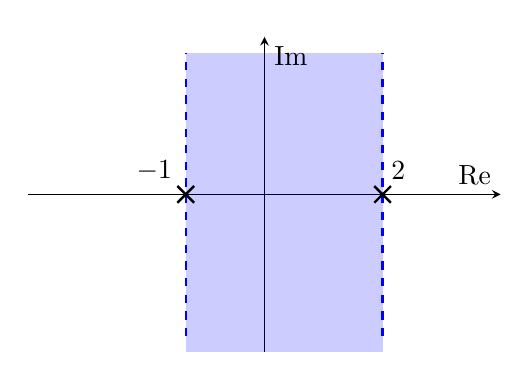
\begin{tikzpicture}
				\begin{axis}
				[
				axis y line=middle,
				axis x line=middle,
				xlabel = {Re},
				ylabel = {Im},
				xtick style={draw=none},
				ytick style={draw=none},
				y=1cm/1,
				x=1cm/1,
				xmin=-3,
				xmax=3,
				ymin=-2,
				ymax=2,
				yticklabels={,,},
				xticklabels={,,},
				%			xtick={1},
				ticklabel style={xshift=0.7ex}
				]
				\draw [name path=A, blue, draw = none, fill = blue, fill opacity = .2](axis cs:-1,-2.8) rectangle (axis cs: 1.5,1.8);
				\draw [blue, thick, dashed] (axis cs: -1,-1.8) -- (axis cs: -1,1.8);
				\draw [blue, thick, dashed] (axis cs: 1.5,-1.8) -- (axis cs: 1.5,1.8);
				\draw (axis cs:-1,0) node {\Cross};
				\draw (axis cs:1.5,0) node {\Cross};
				\draw (axis cs: 1.7,.3) node {$ 2 $};
				\draw (axis cs: -1.4,.3) node {$ -1 $};
				\end{axis}
				
				\end{tikzpicture}
			\end{figure}
		\end{columns}
	}

	\only<6>{
	\begin{columns}
		\column{.5\textwidth}
		For a causal system:
		\[H(s) = \frac{1/3}{s-2} - \frac{1/3}{s+1}\]
		\[h(t) = \frac{1}{3}e^{2t}u(t) - \frac{1}{3}e^{-t}u(t)\]
		
		\column{.5\textwidth}
		\begin{figure}[h!]
			\centering
			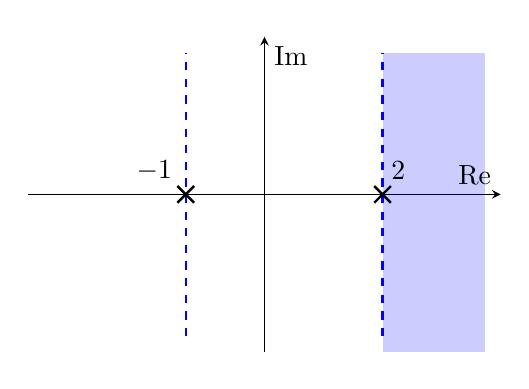
\begin{tikzpicture}
			\begin{axis}
			[
			axis y line=middle,
			axis x line=middle,
			xlabel = {Re},
			ylabel = {Im},
			xtick style={draw=none},
			ytick style={draw=none},
			y=1cm/1,
			x=1cm/1,
			xmin=-3,
			xmax=3,
			ymin=-2,
			ymax=2,
			yticklabels={,,},
			xticklabels={,,},
			%			xtick={1},
			ticklabel style={xshift=0.7ex}
			]
			\draw [name path=A, blue, draw = none, fill = blue, fill opacity = .2](axis cs:1.5,-2.8) rectangle (axis cs: 2.8,1.8);
			\draw [blue, thick, dashed] (axis cs: -1,-1.8) -- (axis cs: -1,1.8);
			\draw [blue, thick, dashed] (axis cs: 1.5,-1.8) -- (axis cs: 1.5,1.8);
			\draw (axis cs:-1,0) node {\Cross};
			\draw (axis cs:1.5,0) node {\Cross};
			\draw (axis cs: 1.7,.3) node {$ 2 $};
			\draw (axis cs: -1.4,.3) node {$ -1 $};
			\end{axis}
			
			\end{tikzpicture}
		\end{figure}
	\end{columns}
}

	\only<7>{
	\begin{columns}
		\column{.5\textwidth}
		For a non-causal and unstable system:
		\[H(s) = \frac{1/3}{s-2} - \frac{1/3}{s+1}\]
		\[h(t) = -\frac{1}{3}e^{2t}u(-t) + \frac{1}{3}e^{-t}u(-t)\]
		
		\column{.5\textwidth}
		\begin{figure}[h!]
			\centering
			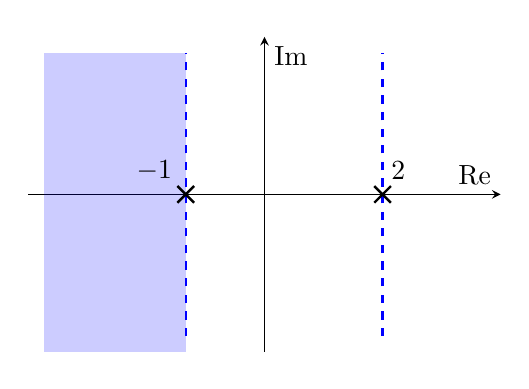
\begin{tikzpicture}
			\begin{axis}
			[
			axis y line=middle,
			axis x line=middle,
			xlabel = {Re},
			ylabel = {Im},
			xtick style={draw=none},
			ytick style={draw=none},
			y=1cm/1,
			x=1cm/1,
			xmin=-3,
			xmax=3,
			ymin=-2,
			ymax=2,
			yticklabels={,,},
			xticklabels={,,},
			%			xtick={1},
			ticklabel style={xshift=0.7ex}
			]
			\draw [name path=A, blue, draw = none, fill = blue, fill opacity = .2](axis cs:-2.8,-2.8) rectangle (axis cs: -1,1.8);
			\draw [blue, thick, dashed] (axis cs: -1,-1.8) -- (axis cs: -1,1.8);
			\draw [blue, thick, dashed] (axis cs: 1.5,-1.8) -- (axis cs: 1.5,1.8);
			\draw (axis cs:-1,0) node {\Cross};
			\draw (axis cs:1.5,0) node {\Cross};
			\draw (axis cs: 1.7,.3) node {$ 2 $};
			\draw (axis cs: -1.4,.3) node {$ -1 $};
			\end{axis}
			\end{tikzpicture}
		\end{figure}
	\end{columns}
}
	\end{frame}

\end{document}